% Format teze zasnovan je na paketu memoir
% http://tug.ctan.org/macros/latex/contrib/memoir/memman.pdf ili
% http://texdoc.net/texmf-dist/doc/latex/memoir/memman.pdf
% 
% Prilikom zadavanja klase memoir, navedenim opcijama se podešava 
% veličina slova (12pt) i jednostrano štampanje (oneside).
% Ove parametre možete menjati samo ako pravite nezvanične verzije
% mastera za privatnu upotrebu (na primer, u b5 varijanti ima smisla 
% smanjiti 
\documentclass[12pt,oneside]{memoir}
% Paket koji definiše sve specifičnosti mastera Matematičkog fakulteta
\usepackage{matfmaster}
%
% Podrazumevano pismo je ćirilica.
%   Ako koristite pdflatex, a ne xetex, sav latinički tekst na srpskom jeziku
%   treba biti okružen sa \lat{...} ili \begin{latinica}...\end{latinica}.
%
% Opicija [latinica]:
%   ako želite da pišete latiniciom, dodajte opciju "latinica" tj.
%   prethodni paket uključite pomoću: \usepackage[latinica]{matfmaster}.
%   Ako koristite pdflatex, a ne xetex, sav ćirilički tekst treba biti
%   okružen sa \cir{...} ili \begin{cirilica}...\end{cirilica}.
%
% Opcija [biblatex]:
%   ako želite da koristite reference na više jezika i umesto paketa
%   bibtex da koristite BibLaTeX/Biber, dodajte opciju "biblatex" tj.
%   prethodni paket uključite pomoću: \usepackage[biblatex]{matfmaster}
%
% Opcija [b5paper]:
%   ako želite da napravite verziju teze u manjem (b5) formatu, navedite
%   opciju "b5paper", tj. prethodni paket uključite pomoću: 
%   \usepackage[b5paper]{matfmaster}. Tada ima smisla razmisliti o promeni
%   veličine slova (izmenom opcije 12pt na 11pt u \documentclass{memoir}).
%
% Naravno, opcije je moguće kombinovati.
% Npr. \usepackage[b5paper,biblatex]{matfmaster}

% Pomoćni paket koji generiše nasumičan tekst u kojem se javljaju sva slova
% azbuke (nema potrebe koristiti ovo u pravim disertacijama)
% Datoteka sa literaturom u BibTex tj. BibLaTeX/Biber formatu

\usepackage{amsthm}
\usepackage[unicode]{hyperref}
\hypersetup{colorlinks,citecolor=green,filecolor=green,linkcolor=blue,urlcolor=blue}

\newtheorem{definic}{Дефиниција}
\bib{master_branislavaz}

% Ime kandidata na srpskom jeziku (u odabranom pismu)
\autor{Бранислава Б. Живковић}
% Naslov teze na srpskom jeziku (u odabranom pismu)
\naslov{Паралелизација статичке верификације софтвера }
% Godina u kojoj je teza predana komisiji
\godina{2016}
% Ime i afilijacija mentora (u odabranom pismu)
\mentor{др Милена \textsc{Вујошевић Јаничић}, доцент\\ Универзитет у Београду, Математички факултет}
% Ime i afilijacija prvog člana komisije (u odabranom pismu)
\komisijaA{др Саша \textsc{Малков}, ванредни професор\\ Универзитет у Београду, Математички факултет}
% Ime i afilijacija drugog člana komisije (u odabranom pismu)
\komisijaB{др Филип \textsc{Марић}, ванредни професор\\ Универзитет у Београду, Математички факултет}
% Ime i afilijacija trećeg člana komisije (opciono)
% \komisijaC{}
% Ime i afilijacija četvrtog člana komisije (opciono)
% \komisijaD{}
% Datum odbrane (obrisati ili iskomentarisati narednu liniju ako datum odbrane nije poznat)
\datumodbrane{ 2016.}

% Apstrakt na srpskom jeziku (u odabranom pismu)
\apstr{%
}

% Ključne reči na srpskom jeziku (u odabranom pismu)
\kljucnereci{паралелизација, верификација, рачунарство}

\begin{document}
% ==============================================================================
% Uvodni deo teze
\frontmatter
% ==============================================================================
% Naslovna strana
\naslovna
% Strana sa podacima o mentoru i članovima komisije
\komisija
% Strana sa posvetom (u odabranom pismu)
\posveta{Брату, мами и тати}
% Strana sa podacima o disertaciji na srpskom jeziku
\apstrakt
\mainmatter
% Sadržaj teze
\tableofcontents

% ==============================================================================
% Glavni deo teze
% ==============================================================================

% ------------------------------------------------------------------------------
%\chapter{Увод}
% ------------------------------------------------------------------------------



\chapter{Увод} 
\subsection{Мотивација}

\chapter{Верификација}
	Верификација софтвера представља дисциплину рачунарства која се бави провером и доказивањем исправности програма. Програм је исправан уколико задовољава задату спецификацију, односно уколико за сваки улаз даје одговарајући излаз предвиђен спецификацијом. Постоје два основна приступа верификацији \emph{динамичка} и \emph{статичка} верификација.
  \section{Динамичка верификација}
  Динамичка верификација се врши током извршавања програма. Грешке у програму се покушавају пронаћи исцрпним тестирањем што је и циљ динамичке верификације. Битно је нагласити да тестирањем није могуће доказати исправност програма већ је могуће пронаћи грешке и на тај начин оповргнути претпоставку о исправности програма. 
  \\ \indent Да би се програм тестирао потребно је пронаћи одговарајући скуп улазних података помоћу којих се врши тестирање.  С обзиром на то да је простор могућих улаза углавном велики, често и превелики, није могуће тестирати програм за све могуће улазе. Због тога треба издвојити одговарајући подскуп улазних података који што боље описује спецификацију програма и покрива што већи број случајева. Избор улазних података се углавном врши коришћењеm програмског кода и спецификације. 
  \\ \indent Постоје две основне методе тестирања, метод \emph{црне} и 
 \emph{беле} кутије.  Методом црне кутије генерисање тестова се врши на основу спецификације програма не узимајући у обзир детаље имплементације. Методом беле кутије тестови се генеришу на основу кода и структуре програма. Такође, постоји и метод сиве кутије који представља мешавину ова два приступа. У зависности од тога шта је потребно тестирати бира/користи се одговарајући метод. 
  
  
  \section{Статичка верификација}
  \section{Алати за верификацију}
  \section{Систем ЛАВ}

\chapter{Паралелизација}
	Термини паралелизам и конкурентност у рачунарству су углавном испреплетани и погрешно схваћени. Често се грешком поистовећују и сматрају синонимима иако то нису. Због тога је битно да их правилно дефинишемо и разликујемо \cite{par_computing}.
\begin{definic}
	Конкурентност је својство програма које се односи на то да два или више задатака могу бити истовремено у току. (исправити превод)
\end{definic}
\begin{definic}
	Паралелизам је својство програма да извршава два или више задатака истовремено. (исправити превод)
\end{definic}

Битно је напоменути да постоји разлика у томе да ли се два задатка истовремено извршавају или су истовремено у току. Наиме, паралелизам изискује/захтева конкурентност, док обрнуто не важи. Може се рећи да је конкурентност начин структуирања програма а паралелизам начин извршавања програма. Конкурентни програми се могу извршавати паралелно али не морају. Паралелизам захтева архитектуру која има више процесорских јединица, док се конкурентност може остварити и на једном процесору.
	\\
 \indent 	Паралелно програмирање је област рачунарства која се бави архитектуром система и софтверским проблемима програма са паралелним извршавањем. Програм се може дефинисати као низ инструкција које се извршавају након његовог покретања. Секвенцијалне програме одликује серијско извршавање инструкција. Паралелизам је карактеристика програма која се односи на независност његових израчунавања. Независна израчунавања се могу истовремено односно паралелно извршавати на више процесорских јединица.
  \section{Мотивација}
  Интересовање за паралелизацију се јавља касних 1950-их са зачетком теоријских основа док се први технички напредак осећа почетком 1960-их и и даље се развија/расте. Први суперрачунари су се појавили 60-их година и имали су више процесора који су могли паралелно да раде са дељеном меморијом. Даљим развојем 80-их година се појављују кластери, системи који се састоје од великог броја рачунара тзв. чворова међусобно повезаних преко мреже. 90-их година са експанзијом интернета се појављује рачунарство у облаку, док данас већина кућних рачунара садржи процесоре са више језгара. \\
  \indent Може се рећи да перформансе рачунара експоненцијално расту од 1945 године за фактор 10 сваких 5 година. Први рачунари су израчунавали десетине операција са бројевима у покретном зарезу у секунди, паралелни рачунари 1990-их достижу број од пар десетина милијарди операција у секунди. Рачунарске/софтверске архитектуре су морале да испрате овакав нагли раст што се постиже преласком са секвенцијалног на паралелно програмирање \cite{par_history}.
  \\
 \indent Перформансе софтверских решења зависе од времена извршавања основних операција, попут операција са бројевима у покретном зарезу, као и од броја оваквих операција које се могу извршавати паралелно. С обзиром на то да ово време зависи од брзине откуцаја часовника процесора која полако тежи ка теоријском максимуму (брзина светлости) не можемо се ослонити на то да ће бржи процесори подићи перформансе нумеричких израчунавања. Главна мотивација и циљ паралелног програмирања је подизање перформанси рачунарских система односно убрзање програма. Потреба за паралелним приступом расте и због тога што је секвенцијалним приступом решавање многих комплексних проблема временски захтевно. 
 \\
\indent \emph{Убрзање паралелизацијом} је мера која показује колико пута паралелни програми брже решавају исте проблеме него секвенцијални програми. Формула убрзања је следећа \cite{par_various}:
 	$$ S = T_s/T_p $$
 	
\noindent где $ T_s $ представља време извршавања секвенцијаног а $ T_p $ време извршавања паралелног програма за исти проблем. 
 	\\
 	\indent По Амдаловом закону, извршавање паралелног програма на паралелном рачунару углавном обухвата и део операција које се не могу извршавати паралелно. Означимо са $ \alpha $ део програма који се мора извршавати секвенцијално на једном процесору, а остатак $ (1 - \alpha)$ се може извршити паралелно. Ако је $ N $ број процесорских јединица, формула убрзања је: 
 	$$ S = 1 / ( \alpha + (1-\alpha)/N)$$
Ова формула нам показује да убрзање никада не може прећи $ 1/\alpha $, тј. број процесорских јединица не утиче на део програма који се мора извршавати секвенцијално. На слици \ref{fig:amdal} је приказана зависност убрзања од броја процесора и дела посла који се мора обавити секвенцијално.

 \begin{figure}[!ht]
  \centering
  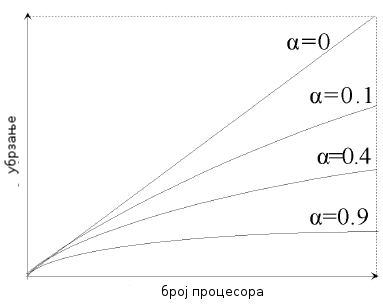
\includegraphics[width=0.8\textwidth]{amdal.png}
  \caption{Зависност убрзања од броја процесора за неке вредности $ \alpha $ }
  \label{fig:amdal}
\end{figure}


 \indent У пракси, време извршавања програма на паралелним системима је углавном веће од теоријски израчунате вредности јер зависи и од других параметара попут комуникације и синхронизације. Амдалов модел не узима у обзир ова времена и разматра само случајеве у којима је димензија проблема фиксирана. Поред Амдаловог модела постоје и други модели као што су Густафсонов, Гинтеров, модел Сун Ни-ја који превазилазе нека ограничења Амдаловог модела \cite{performance}.
 	 


  \section{Врсте паралелизације}
  
 Програми се могу паралелизовати на различите начине. Паралилзацију може обављати програмер експлицитно или коришћењем неких алата. Последњих година развијени су многи алати који омогућују аутоматску паралелизацију. Коришћењем ових алата програмеру је олакшан процес паралелизације уз ограничену контролу. Овакав начин паралелизације је погодан за велике и комплексне системе код којих би ручна паралелизација била спора и компликована.
 \\
 \indent Са друге стране, ручна паралелизација програма захтева добро обучене програмере и углавном је сложенија али пружа програмерима потпуну контролу над самим процесом паралелизације. Овакав приступ је погоднији за паралелизацију специфичних проблема.
 \\
  \indent  Битно је нагласити да није могуће паралелизовати све делове сваког алгоритма. Посао програмера је да пронађе и одлучи који делови алгоритма се могу паралелизовати и на који начин.
 Два најчешћа приступа дизајнирању паралелних алгоритама су \emph{паралелизација задатака} и \emph{паралелизација података}. 
Паралелизација задатака представља раслојавање алгоритма на независне задатке који се могу извршавати било којим редоследом над истим скупом података.
Паралелизација података представља раслојавање података тако да се један задатак може независно извршавати над дисјунктним деловима података било којим редоследом \cite{art_conc}. 
На слици  \ref{fig:data_parallel} је приказан пример паралелизације задатака а на слици \ref{fig:task_parallel} пример паралелизације података

\begin{figure}[!ht]
  \centering
  \includegraphics[width=0.96\textwidth]{data_parallel.png}
  \caption{Пример паралелизације података: примена функције capslock над сваким словом појединачно}
  \label{fig:data_parallel}
\end{figure}

\begin{figure}[!ht]
  \centering
  \includegraphics[width=0.96\textwidth]{task_parallel.png}
  \caption{Пример паралелизације задатака: примена различитих функција над свим подацима}
  \label{fig:task_parallel}
\end{figure}


  \section{Проблеми}
  Често није могуће раслојити алгоритам на потпуно независне задатке који се могу паралелно извршавати већ је присутан одређен ниво зависности између њих. На пример, уколико задаци могу приступити истој променљивој у програму и променити њену вредност, потенцијално више задатака може истовремено покушати да је измени. У таквим ситуацијама задаци се надмећу за приступ дењеним подацима.  Овакви и овоме слични проблеми индукују постојање \emph{критичне секције}. Критична секција представља низ инструкција који мора задовољавати следећи услов: уколико је један задатак ушао у критичну секцију и почео да је извршава, ниједан други задатак је не сме извршавати истовремено. У складу са тиме постоје бројна решења и механизми који омогућавају \emph{комуникацију} и  \emph{синхронизацију} између задатака.
\\ 
 \indent  
Комуникација представља било који вид размене информација између задатака. Може се остварити преко дељене меморије или слањем односно примањем порука. Комуникација преко порука се одвија тако што један задатак експлицитно шаље податке другом задатку који их прихвата и обрађује. Неки од познатих механизама за овакав вид комуникације су сигнали, цеви, сокети и канали.
Постојање дељене меморије има своје добре и лоше стране. Понекад је потребно старати се о редоследу читања односно писања дељене меморије као и о евентуалним утркивањима и сукобима. Због тога комуникација преко дељене меморије може захтевати одређен ниво синхронизације. Кроз механизме синхронизације програмер може контролисати редослед извршавања задатака и приступ дељеној меморији. Две основне врсте овакве синхронизације су \emph{сарадња} и \emph{такмичење}. Синхронизација сарадње између два задатка је потребна уколико један задатак зависи од резултата рада другог. Синхронизација такмичења је неоходна у случајевима када два задатка истовремено захтевају исти ресурс. Механизми који се користе за имплементацију синхронизације су мутекси, катанци, семафори, монитори и други. \cite{lang_prag}
\\ \indent Синхронизација отвара (нека друга реч ?)  могућност узајамног блокирања, живог блокирања и изгладњивања између задатака. Ови проблеми се односе на концепт напредовања (енг. liveness) програма. Концепт напредовања програма представља својство програма да у току свог извршавања напредује доводећи до завршетка рада у неком тренутку, односно да константно прави прогрес током свог извршавања. Уколико ово својство није задовољено може да се деси да програм никада не заврши свој рад. Поменути проблеми се могу јавити управо у оваквим ситуацијама.

Prilikom paralelizacije programa posebno je vazno obratiti paznju na mogucnost uzajamnog blokiranja, zivog blokiranja i izglasnjivanja izmedju zadataka. Ovi problemi se odnose na koncept koji se javlja  
svojstvo programa da napreduje u toku svog izvrsavanja

 % \section{Неки патерни}
  \section{Алати за паралелизацију}
	У овом поглављу ће бити описане неке библиотеке које се користе за паралелизацију програмског кода. Акценат ће бити на библиотекама за језик Ц++. 
	\\ \indent Алате можемо поделити у две категорије имплицитне и експлицитне. Имплицитни алати олакшавају програмеру имплементацију паралелних алгоритама јер се старају о прављењу, управљању и синхронизацији нити. Експлицитни алати пружају већу флексибилности и контролу захтевајући од програмера да управља свим аспектима вишенитности.
	
\paragraph{ PThreads (енг. POSIX Threading interface)} је интерфејс за паралелно програмирање на нивоу оперативног система и доступан је у оквиру већине UNIX-оликих оперативних система. Имплементиран је у оквиру заглавља \\ \texttt{pthread.h} језика Ц који садржи скуп константи, типова и функција за паралелизацију. Програмеру је омогућено прављење нити и управљање њиховим извршавањем. Комуникација се обавља преко дељене меморије коју такође програмер контролише. Дељена меморија се имплементира коришћењем глобалних променљивих које су видљиве свим нитима. Садржај заглавља \texttt{pthread.h} уз одговарајућу документацију се може наћи на адреси \url{http://man7.org/linux/man-pages/man7/pthreads.7.html}.

\paragraph{OpenMP (енг. Open Specification for Multi-Processing)} је интерфејс за програмирање који омогућава паралелно програмирање у језицима Ц, Ц++ и Фортран . Заснива се на моделу паралелизације коришћењем дељене меморије. Садржи скуп компајлерских директива, рутина и глобалних променљивих које служе за обележавање делова програмског кода. Програм се дели на регионе који се извршавају серијски и регионе који се извршавају паралелно. Региони се означавају директивама које управљају процесом додељивања задатака нитима, комуникацијом и синхронизацијом. Променљиве могу бити дељене, односно видљиве свим нитима, и приватне, односно видљиве у оквиру нити унутар које су декларисане. Детаљна документација се може наћи на адреси \url{http://www.openmp.org}. 

\paragraph{TBB (енг. Thread Building Blocks)} је Ц++ библиотека за паралелно програмирање на вишепроцесорским системима развијена од стране \emph{Intel}-а. Библиотека се састоји од бројних шаблона који имплементирају паралелне алгоритме, контејнере, примитиве за синхронизацију и управљач задацима. Програмери дефинишу задатке који ће се извршавати паралелно након чега се управљач задацима стара о току извршавања и техничким детаљима. Више о овој библиотеци се може наћи на адреси \url{http://www.threadingbuildingblocks.org}.


  
\chapter{Имплементација}
Mодул који се бави паралелизацијом је развијен у складу са специфичним захтевима система ЛАВ. Систем ЛАВ је сложен верификациони алат писан у Ц++ језику. Као такав користи многе екстерне (спољне ?) библиотеке, алате, као и СМТ решаваче.  Архитектура самог система је модуларна, функционалне целине су издвојене у посебне модуле и по потреби увезиване и коришћене. Модул за паралелизацију представља посебну издвојену целину тако да се може универзално користити у различитим деловима система. Имплементиран је коришћењем  и комбинацијом различитих библиотека језика Ц++.   У наставку текста ће бити описана архитекура и имплементација модула за паралелизацију као и начини његовог коришћења у оквиру система ЛАВ.
\section{Опис архитектуре}

Архитектура модула за паралелизацију је осмишљена тако да испуњава захтеве система ЛАВ. Модул за паралелизацију има три основна дела: контролни део, радне нити и комуникациони део. Улога контролног дела је да управља радним нитима, ослушкује и прихвата сигнале тј. догађаје које емитују радне нити и обрађује 	њихове резултате. Радне нити извршавају задатке и обавештавају контролни део о резултатима. Део који се бави комуникацијом омогућава комуникацију између контролног дела и радних нити.  Композицијом ових делова имплементиран је модул који паралелизује неке делове алгоритма анализе програмског кода у овиру система ЛАВ.
\newpage

\section{Имплементација модула}
За имплементацију модула коришћен је језик Ц++ због компатибилности са системом ЛАВ. Приликом имплементације појединачних нити коришћен је модел нити из библиотеке \texttt{<thread>} језика Ц++. Ова библиотека је јавно доступнa и нуди интерфејс (енг. application programming interface, API) за конструкцију и управљање нитима. 
\\ \indent 
Класа \texttt{ThreadPool} представља контролни део модула, тзв. базен нити. Она садржи контролну нит чија је улога контрола радних нити које се такође налазе у оквиру ове класе (\texttt{ThreadPool}). Посао радних нити је да извршавају задатке који су прослеђени базену нити. Због тога се унутар базена нити чува и ред задатака (класа \texttt{FixedQueue}) које је потребно извршити. Класа \texttt{FixedQueue} је шаблонска класа и може садржати ред објеката било ког типа. Задаци који се смештају у ред су објекати Ц++ апстракције анонимних (ламбда) функција, и због специфичности проблема имају следећи потпис: \texttt{int f()}. Наравно, потпис ових функција се може уопштити, али за потребе овог рада то није било неопходно. 
\\ \indent 
 Задатке извршавају радне нити, објекти класе \texttt{std::thread}, које су обмотане класом \texttt{SignalingThread}.
 Класа \texttt{std::thread} (која постоји у оквиру Ц++ библиотеке \texttt{<thread>})  нуди многобројне корисне функције за рад са нитима и  као што су нпр. \texttt{join, detach, joinanble,...} Базен нити садржи објекат реда \texttt{FixedQueue} као и низ радних нити. Могуће је задати број нити али уколико другачије није наглашено конструисаће се онолико радних нити колико оперативни систем дозвољава.
 \\ \indent
Свакој радној нити се приликом иницијализације прослеђује дељени показивач (\texttt{std::shared\_ptr}) на ред задатака, тако да све нити имају приступ истом објекту реда. Нити скидају са реда један по један задатак и извршавају га. Како све нити приступају истом објекту реда, потребно је синхронизовати процес скидања задатака. Ц++ језик, у оквиру библиотеке \texttt{<atomic>} нуди разне типове над којим су подржане атомичне операције. Све операције над овим типовима су безбедне у контексту вишенитног окружења. Класа \texttt{FixedQueue} садржи јединствен показивач на објекат атомичног типа (\texttt{std::unique\_ptr<std::atomic\_uint>}). Овај објекат садржи цео број и чува информацију о томе колико је задатака скинуто са реда (индекс следећег задатка који треба скинути). У тренутку када радна нит затражи задатак из реда позива се функција \texttt{fetch\_add} над овим објектом. Функција  \texttt{fetch\_add} враћа вредност објекта (цео број) и након тога увећава његову вредност, обезбеђујући атомичност ових операције. Уколико две или више нити у исто време покушају скинути задатак са реда, свака ће добити различит задатак. Тако да се приликом испоруке задатака гарантује да ће све нити добити различите задатке.  На овај начин је избегнуто утркивање нити као и синхронизација коришћењем традиционалних метода (мутекси, закључавање, и др). 
\\ \indent 
Након што изврши задатак, нит обавештава базен нити емитовањем догађаја, објекат класе  \texttt{Event}. Свака нит садржи посебан објекат догађаја тако да се базен нити претплаћује на ослшкивање догађаја сваке нити посебно. Резултат извршавања задатака нити обрађују и шаљу сигнал базену нити емитовањем одговарајућег догађаја. Контролна нит која се налази у базену нити тумачи сигнал и предузима потребне акције. 
 
\section{Интеграција модула са системом ЛАВ}

Паралелизација је имплементирана у контексту анализе блока програмског кода. Класа \texttt{LBlock} система ЛАВ служи за рад са блоковима кода. Њена функција \texttt{CalculateConditions} конструише формуле које представљају услове исправности блока и позивају SMT решавач за сваку формулу. Модул за паралелизацију омогућава да се ови позиви решавача извршавају паралелно.
\\ \indent 
 За сваку формулу, услов исправности, унутар функције \texttt{CalculateConditions} конструише се анонимна функција која позива SMT решавач. Анонимна функција као резултат враћа индикатор да ли је услов исправности испуњен или не. Направљене функције се смештају у ред \texttt{FixedQueue} и прослеђују инстанци класе \texttt{ThreadPool} (базен нити). Базен нити прави радне нити и покреће их. Свака нит извршава једну по једну анонимну функцију, скидајући их са реда и обавештава базен нити о резултату извршавања. Уколико се наиђе на услов исправности који није задовољен, нема потребе испитивати остале услове јер се тада блок сматра неисправним. У контексту имплементације то значи да уколико нека анонимна функција врати индикатор да услов исправности није испуњен, нити могу престати са радом јер се задат блок означава као неисправан. Ако је приликом покретања система ЛАВ (била) задата опција \texttt{-find-first-flawed} базен нити у таквој ситуацији зауставља све нити. У супротном нити настављају са радом. Уколико су све функције из реда извршене и сви услови су били задовољени, блок се сматра исправним и тако бива означен. 
 \\ \indent
 На слици \ref{fig:sekv_dij}  је приказан један могући сценарио. На почетку се врши конструкција и иницијализација свих потребних објеката. Базен нити конструише три радне нити које узимају задатке са реда. Нити  \texttt{SignalingThread1} прва узима задатак са реда, а након ње и \texttt{SignalingThread2} и обе почињу да их извршавају. Нит \texttt{SignalingThread1} прва завршава успешно, пре него што је нит \texttt{SignalingThread3} узела задатак са реда. Након тога обе нити,  \texttt{SignalingThread1} и  \texttt{SignalingThread3} покушају узети следећи задатак. Имајући у виду то да један ред задатака деле све нити, овај процес узимања задатака ће се извршити секвенцијално (користећи погодне функције из библиотеке  \texttt{<atomic>}) тако да нит \texttt{SignalingThread1} прва добија задатак са реда. Како нит  \texttt{SignalingThread1} наилази на услов исправности који није испуњен, шаље сигнал базену нити након чега остале нити бивају заустављене и систем ЛАВ бива обавештен о неисправном резултату. Можемо приметити да је редослед акција прављења нити, узимање задатака са реда и брзина извршавања задатака у овом примеру конкретизован. Наравно, у општем случају тај редослед је произвољан и зависи од много фактора као што су специфичности оперативног система, сложеност задатака, број задатака у реду, и слично.  

\begin{figure}[!ht]
  \centering
  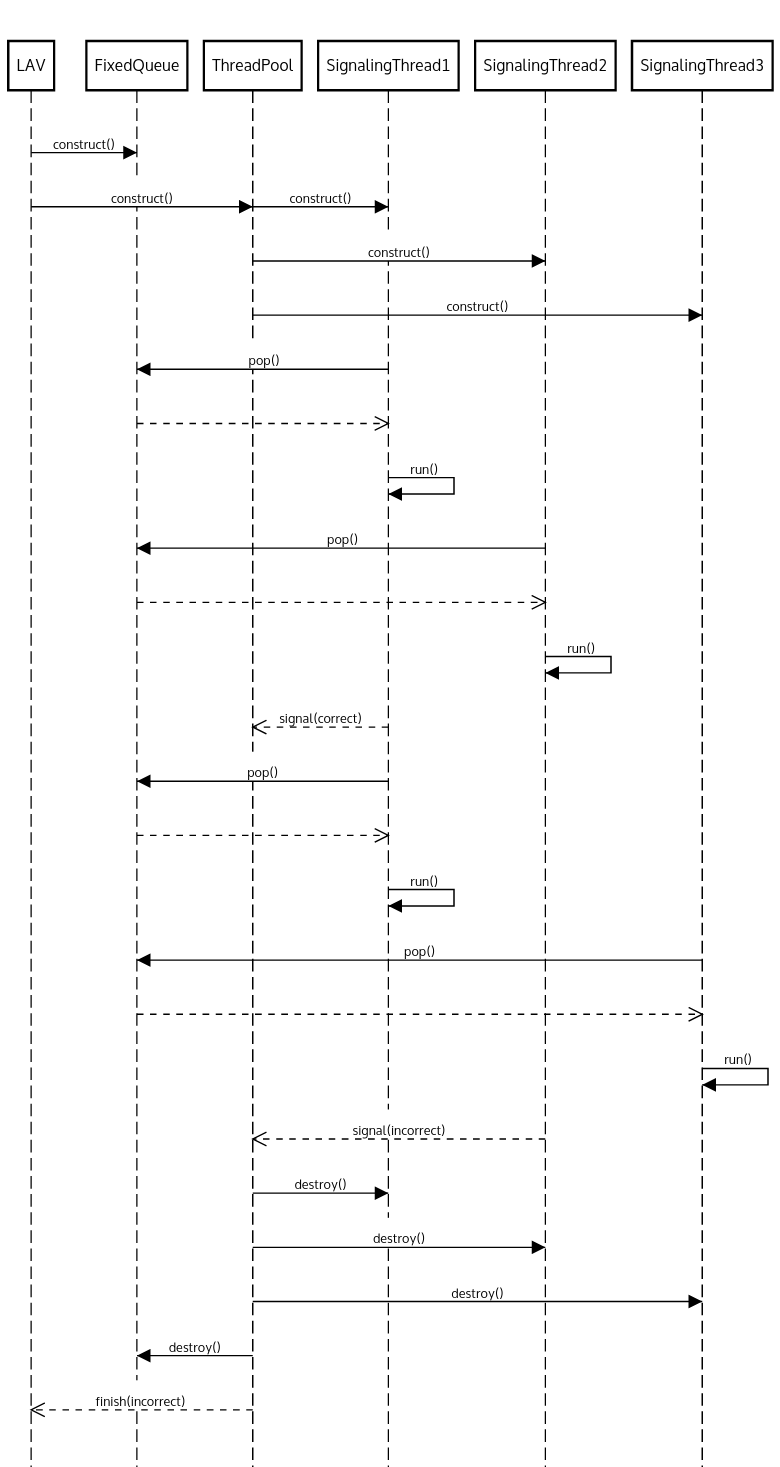
\includegraphics[width=0.8\textwidth]{sekvencijalni_dijagram.png}
  \caption{Дијаграм тока извршавања}
  \label{fig:sekv_dij}
\end{figure}

\chapter{Експериментални резултати}
  \section{Архитектура рачунара}
  \section{Опис корпуса}
  \section{Начини покретања}
  \section{Измерена времена}
 \section{Објашњавање експерименталних резултата}

\literatura
% ==============================================================================
% Završni deo teze i prilozi
\backmatter
\end{document} 
